\section{Motivation and Scope}

There has been a strong desire for a more space- and/or runtime-efficient
representation for \code{map} among C++ users for some time now.  This has
motivated discussions among the members of SG14, numerous articles and talks,
and an implementation in Boost, \code{boost::container::flat_map}.  Virtually
everyone who makes games, embedded, or system software in C++ uses the Boost
implementation or one that they rolled themselves.\\

Here are some numbers that show why.  The graphs that follow show runtimes for
different \code{map}-like associative containers.  The containers used are
Boost.FlatMap, \code{std::map}, and two thin wrappers over a sorted
\code{std::vector}; the ``custom pair'' version of the sorted
\code{std::vector} uses a simple \code{struct} instead of \code{std::pair} for
its value type.  All containers use an \code{int} as the key type and an
\code{int} or a \code{struct} with 5 \code{double}s for the value type.\\

These first three graphs cover the \code{int}-value-type case.  The first
graph shows insertion of N elements with random keys; the second shows full
iteration across all N elements; and the third shows erasure of all N
elements, by the keys used in the original insertions.

\begin{center}
    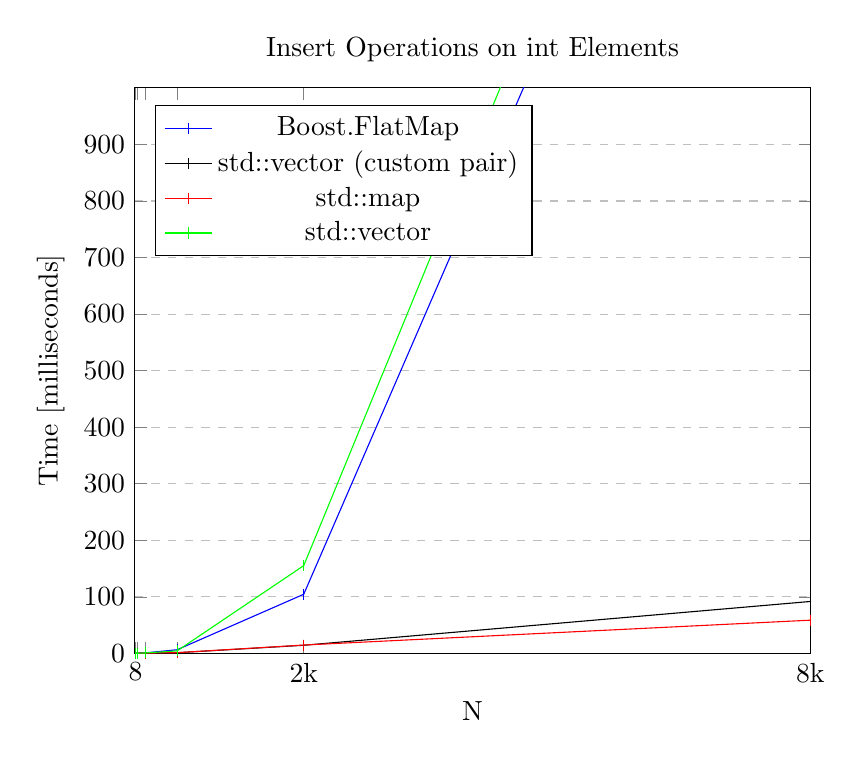
\begin{tikzpicture}
    \begin{axis}[
        width=4in,
        title={Insert Operations on int Elements},
        xlabel={N},
        ylabel={Time [milliseconds]},
        xmin=0, xmax=8192.0,
        ymin=0, ymax=1000.0,
        xtick={8,32,128,512,2048,8192},
        xticklabels={8,,,,2k,8k},
        ytick={0.0,100.0,200.0,300.0,400.0,500.0,600.0,700.0,800.0,900.0},
        legend pos=north west,
        ymajorgrids=true,
        grid style=dashed,
        scaled x ticks=false,
        legend entries={Boost.FlatMap,std::vector (custom pair),std::map,std::vector},
        ]

    \addplot[color=blue,mark=|,]
        coordinates {(8,0.088279)(32,0.269867)(128,0.896692)(512,6.36352)(2048,104.485)(8192,2168.83)};

    \addplot[color=black,mark=|,]
        coordinates {(8,0.073962)(32,0.112724)(128,0.408641)(512,1.14889)(2048,14.2758)(8192,91.7388)};

    \addplot[color=red,mark=|,]
        coordinates {(8,0.073123)(32,0.225377)(128,0.484908)(512,1.17082)(2048,14.6917)(8192,58.6582)};

    \addplot[color=green,mark=|,]
        coordinates {(8,0.067397)(32,0.141638)(128,0.7656)(512,4.29852)(2048,155.133)(8192,2333.62)};

    \end{axis}
\end{tikzpicture}
\end{center}

\begin{center}
    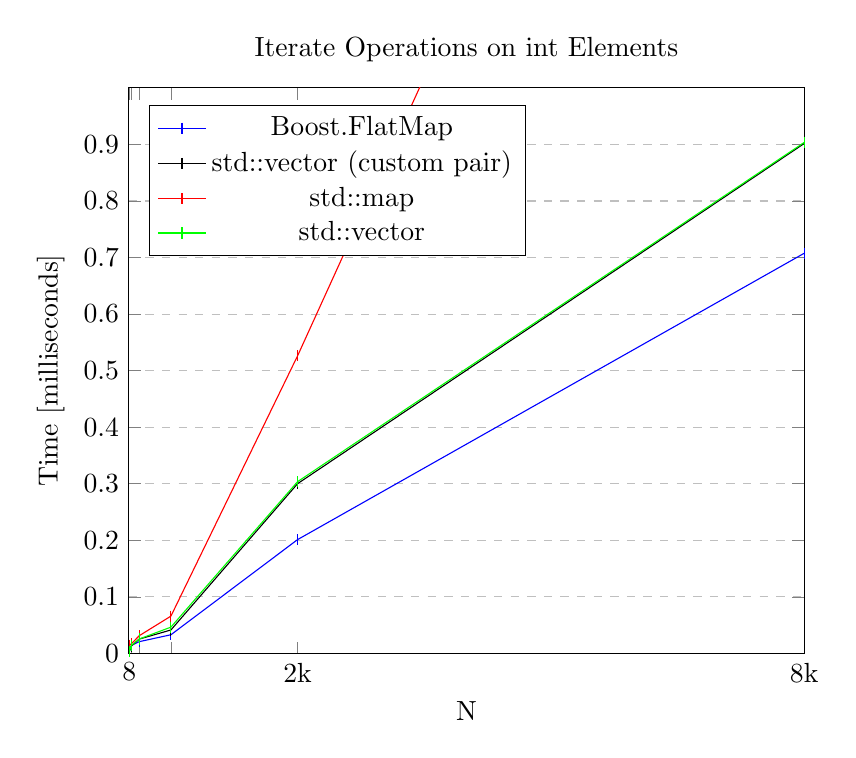
\begin{tikzpicture}
    \begin{axis}[
        width=4in,
        title={Iterate Operations on int Elements},
        xlabel={N},
        ylabel={Time [milliseconds]},
        xmin=0, xmax=8192.0,
        ymin=0, ymax=1.0,
        xtick={8,32,128,512,2048,8192},
        xticklabels={8,,,,2k,8k},
        ytick={0.0,0.1,0.2,0.3,0.4,0.5,0.6,0.7,0.8,0.9},
        legend pos=north west,
        ymajorgrids=true,
        grid style=dashed,
        scaled x ticks=false,
        legend entries={Boost.FlatMap,std::vector (custom pair),std::map,std::vector},
        ]

    \addplot[color=blue,mark=|,]
        coordinates {(8,0.003562)(32,0.014108)(128,0.020673)(512,0.032895)(2048,0.201143)(8192,0.707493)};

    \addplot[color=black,mark=|,]
        coordinates {(8,0.003632)(32,0.01285)(128,0.025213)(512,0.041346)(2048,0.300039)(8192,0.901582)};

    \addplot[color=red,mark=|,]
        coordinates {(8,0.014387)(32,0.016902)(128,0.03122)(512,0.06586)(2048,0.526114)(8192,2.49543)};

    \addplot[color=green,mark=|,]
        coordinates {(8,0.003632)(32,0.013968)(128,0.025422)(512,0.046375)(2048,0.3036)(8192,0.903467)};

    \end{axis}
\end{tikzpicture}
\end{center}

\begin{center}
    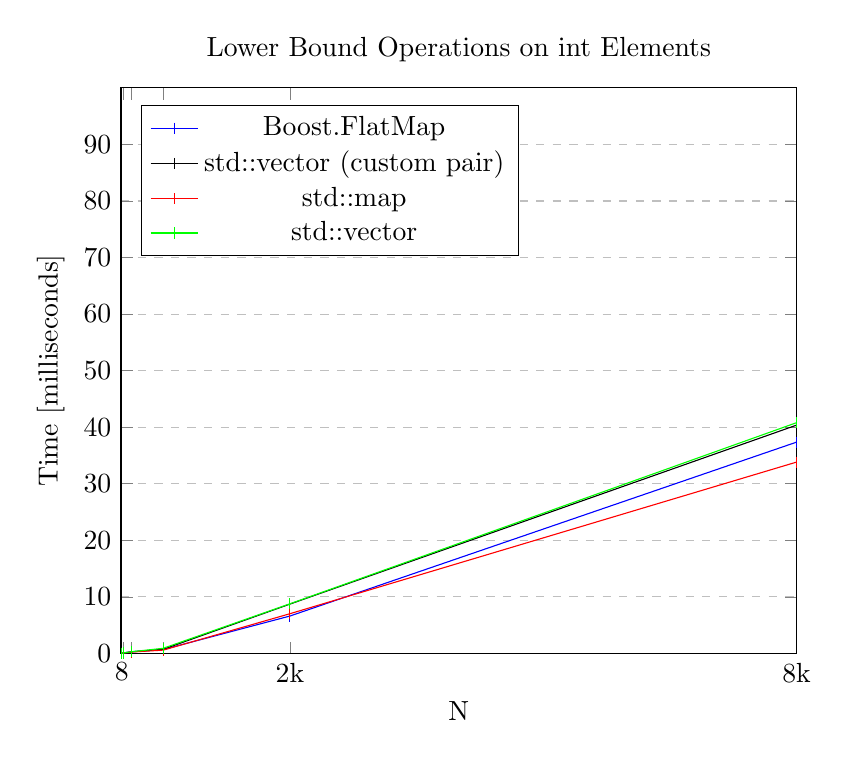
\begin{tikzpicture}
    \begin{axis}[
        width=4in,
        title={Lower Bound Operations on int Elements},
        xlabel={N},
        ylabel={Time [milliseconds]},
        xmin=0, xmax=8192.0,
        ymin=0, ymax=100.0,
        xtick={8,32,128,512,2048,8192},
        xticklabels={8,,,,2k,8k},
        ytick={0.0,10.0,20.0,30.0,40.0,50.0,60.0,70.0,80.0,90.0},
        legend pos=north west,
        ymajorgrids=true,
        grid style=dashed,
        scaled x ticks=false,
        legend entries={Boost.FlatMap,std::vector (custom pair),std::map,std::vector},
        ]

    \addplot[color=blue,mark=|,]
        coordinates {(8,0.027169)(32,0.096521)(128,0.276921)(512,0.675016)(2048,6.59581)(8192,37.3482)};

    \addplot[color=black,mark=|,]
        coordinates {(8,0.027238)(32,0.065022)(128,0.280273)(512,0.720274)(2048,8.70921)(8192,40.353)};

    \addplot[color=red,mark=|,]
        coordinates {(8,0.022699)(32,0.081155)(128,0.231594)(512,0.571721)(2048,7.00634)(8192,33.819)};

    \addplot[color=green,mark=|,]
        coordinates {(8,0.030102)(32,0.067816)(128,0.288165)(512,0.895226)(2048,8.76403)(8192,40.7894)};

    \end{axis}
\end{tikzpicture}
\end{center}

\begin{center}
    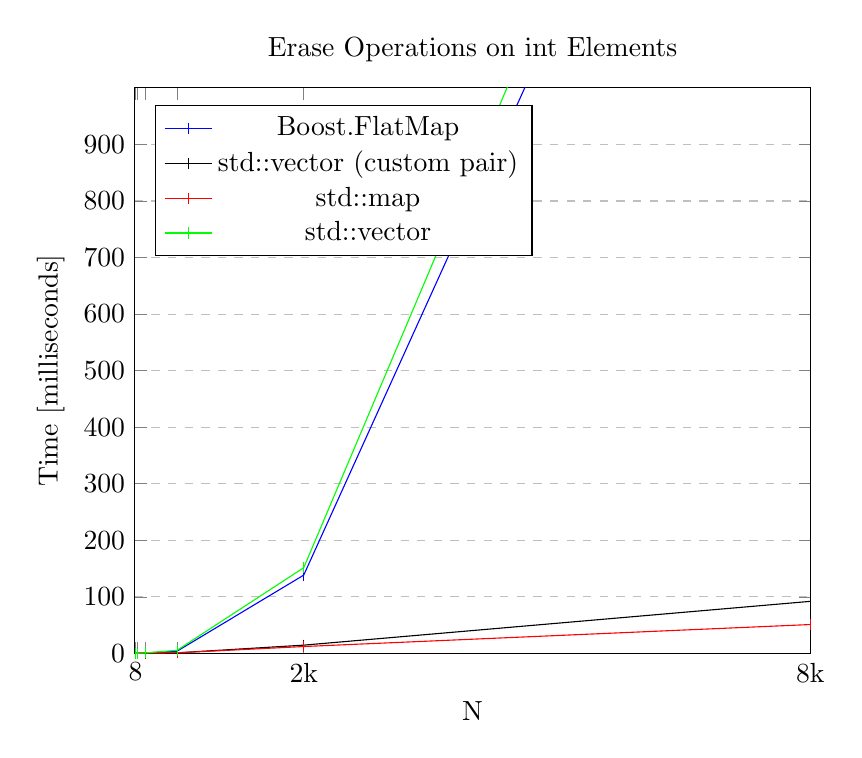
\begin{tikzpicture}
    \begin{axis}[
        width=4in,
        title={Erase Operations on int Elements},
        xlabel={N},
        ylabel={Time [milliseconds]},
        xmin=0, xmax=8192.0,
        ymin=0, ymax=1000.0,
        xtick={8,32,128,512,2048,8192},
        xticklabels={8,,,,2k,8k},
        ytick={0.0,100.0,200.0,300.0,400.0,500.0,600.0,700.0,800.0,900.0},
        legend pos=north west,
        ymajorgrids=true,
        grid style=dashed,
        scaled x ticks=false,
        legend entries={Boost.FlatMap,std::vector (custom pair),std::map,std::vector},
        ]

    \addplot[color=blue,mark=|,]
        coordinates {(8,0.049029)(32,0.182076)(128,0.732076)(512,3.80041)(2048,138.355)(8192,2113.37)};

    \addplot[color=black,mark=|,]
        coordinates {(8,0.043372)(32,0.085904)(128,0.359194)(512,0.930635)(2048,14.5091)(8192,91.9592)};

    \addplot[color=red,mark=|,]
        coordinates {(8,0.053638)(32,0.115727)(128,0.380914)(512,0.914012)(2048,12.0617)(8192,50.9554)};

    \addplot[color=green,mark=|,]
        coordinates {(8,0.052241)(32,0.121384)(128,0.737175)(512,5.42716)(2048,151.442)(8192,2266.69)};

    \end{axis}
\end{tikzpicture}
\end{center}


These next three graphs are just like the preceding ones, but cover the
\code{struct}-value-type case.

\begin{center}
    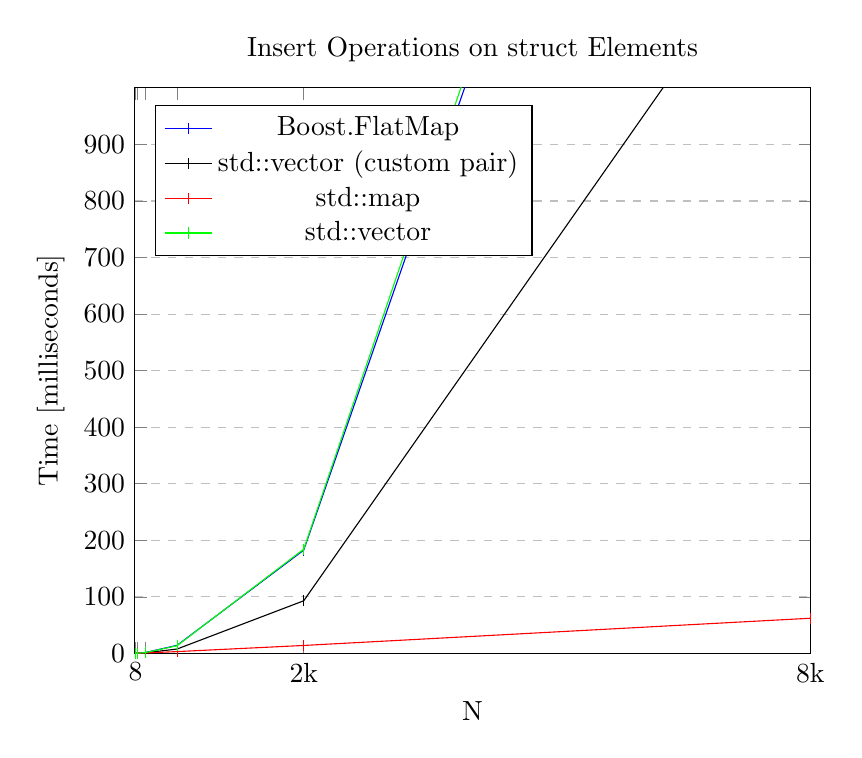
\begin{tikzpicture}
    \begin{axis}[
        width=4in,
        title={Insert Operations on struct Elements},
        xlabel={N},
        ylabel={Time [milliseconds]},
        xmin=0, xmax=8192.0,
        ymin=0, ymax=1000.0,
        xtick={8,32,128,512,2048,8192},
        xticklabels={8,,,,2k,8k},
        ytick={0.0,100.0,200.0,300.0,400.0,500.0,600.0,700.0,800.0,900.0},
        legend pos=north west,
        ymajorgrids=true,
        grid style=dashed,
        scaled x ticks=false,
        legend entries={Boost.FlatMap,std::vector (custom pair),std::map,std::vector},
        ]

    \addplot[color=blue,mark=|,]
        coordinates {(8,0.069283)(32,0.280622)(128,1.54419)(512,14.175)(2048,182.555)(8192,2756.55)};

    \addplot[color=black,mark=|,]
        coordinates {(8,0.049518)(32,0.167689)(128,0.918134)(512,7.64839)(2048,92.9722)(8192,1372.1)};

    \addplot[color=red,mark=|,]
        coordinates {(8,0.046095)(32,0.160565)(128,0.685981)(512,3.09634)(2048,13.9592)(8192,62.0826)};

    \addplot[color=green,mark=|,]
        coordinates {(8,0.050076)(32,0.213854)(128,1.32873)(512,13.5)(2048,184.269)(8192,2814.09)};

    \end{axis}
\end{tikzpicture}
\end{center}

\begin{center}
    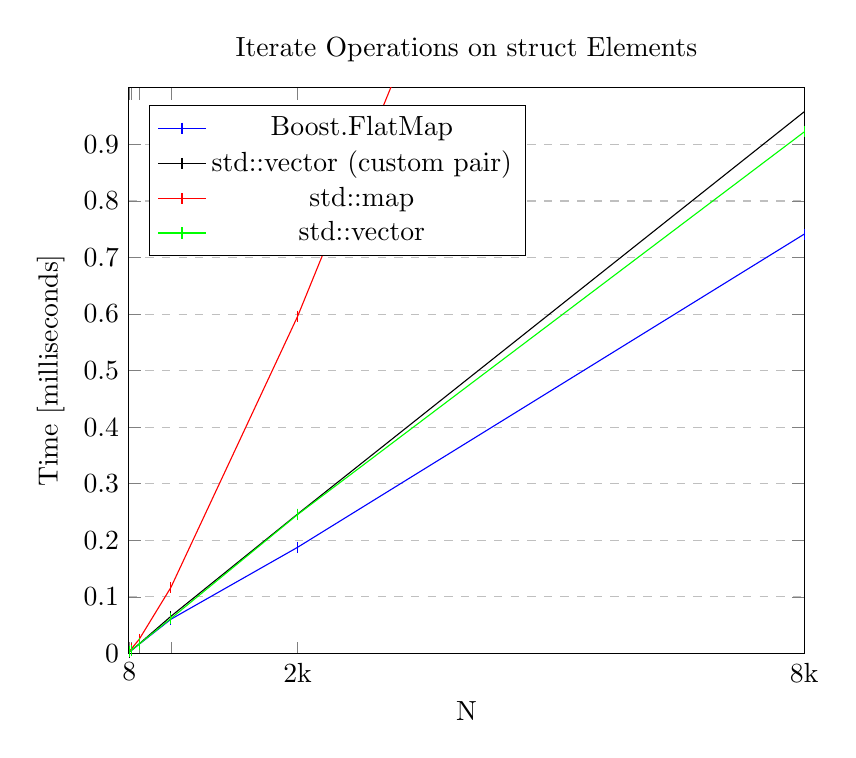
\begin{tikzpicture}
    \begin{axis}[
        width=4in,
        title={Iterate Operations on struct Elements},
        xlabel={N},
        ylabel={Time [milliseconds]},
        xmin=0, xmax=8192.0,
        ymin=0, ymax=1.0,
        xtick={8,32,128,512,2048,8192},
        xticklabels={8,,,,2k,8k},
        ytick={0.0,0.1,0.2,0.3,0.4,0.5,0.6,0.7,0.8,0.9},
        legend pos=north west,
        ymajorgrids=true,
        grid style=dashed,
        scaled x ticks=false,
        legend entries={Boost.FlatMap,std::vector (custom pair),std::map,std::vector},
        ]

    \addplot[color=blue,mark=|,]
        coordinates {(8,0.002445)(32,0.005168)(128,0.016343)(512,0.060343)(2048,0.187524)(8192,0.741295)};

    \addplot[color=black,mark=|,]
        coordinates {(8,0.002375)(32,0.005378)(128,0.016832)(512,0.065511)(2048,0.24626)(8192,0.957664)};

    \addplot[color=red,mark=|,]
        coordinates {(8,0.003142)(32,0.007752)(128,0.025003)(512,0.116705)(2048,0.595816)(8192,2.7954)};

    \addplot[color=green,mark=|,]
        coordinates {(8,0.002514)(32,0.005378)(128,0.016552)(512,0.06167)(2048,0.245353)(8192,0.922045)};

    \end{axis}
\end{tikzpicture}
\end{center}

\begin{center}
    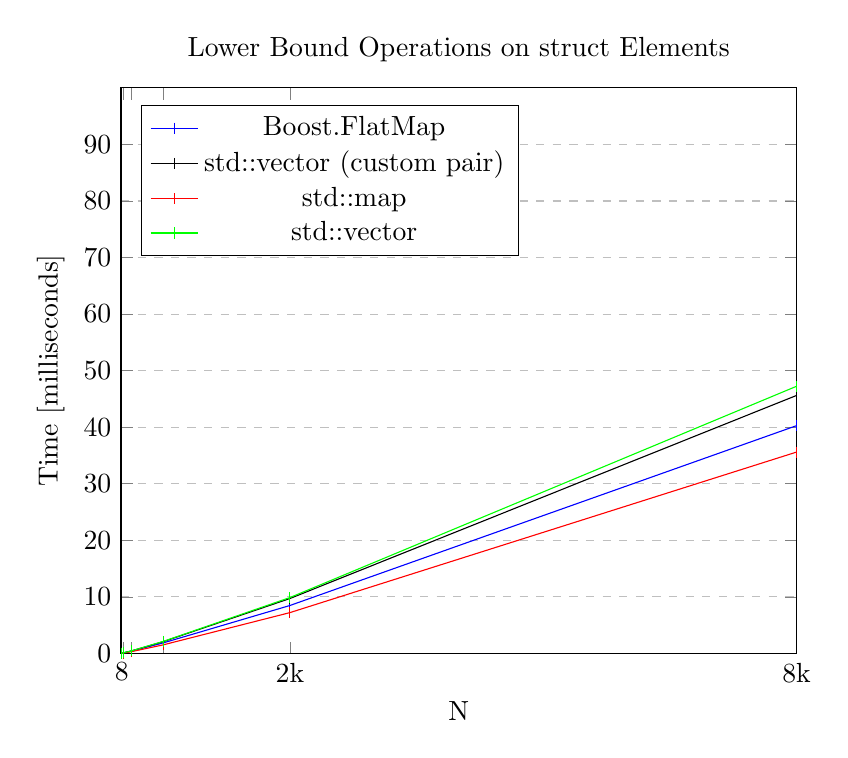
\begin{tikzpicture}
    \begin{axis}[
        width=4in,
        title={Lower Bound Operations on struct Elements},
        xlabel={N},
        ylabel={Time [milliseconds]},
        xmin=0, xmax=8192.0,
        ymin=0, ymax=100.0,
        xtick={8,32,128,512,2048,8192},
        xticklabels={8,,,,2k,8k},
        ytick={0.0,10.0,20.0,30.0,40.0,50.0,60.0,70.0,80.0,90.0},
        legend pos=north west,
        ymajorgrids=true,
        grid style=dashed,
        scaled x ticks=false,
        legend entries={Boost.FlatMap,std::vector (custom pair),std::map,std::vector},
        ]

    \addplot[color=blue,mark=|,]
        coordinates {(8,0.021581)(32,0.091492)(128,0.404172)(512,1.84709)(2048,8.46113)(8192,40.2611)};

    \addplot[color=black,mark=|,]
        coordinates {(8,0.01725)(32,0.093587)(128,0.436857)(512,2.07093)(2048,9.6969)(8192,45.6048)};

    \addplot[color=red,mark=|,]
        coordinates {(8,0.018787)(32,0.063695)(128,0.301016)(512,1.50389)(2048,7.20106)(8192,35.5892)};

    \addplot[color=green,mark=|,]
        coordinates {(8,0.025422)(32,0.094356)(128,0.442095)(512,2.11375)(2048,9.86641)(8192,47.2265)};

    \end{axis}
\end{tikzpicture}
\end{center}

\begin{center}
    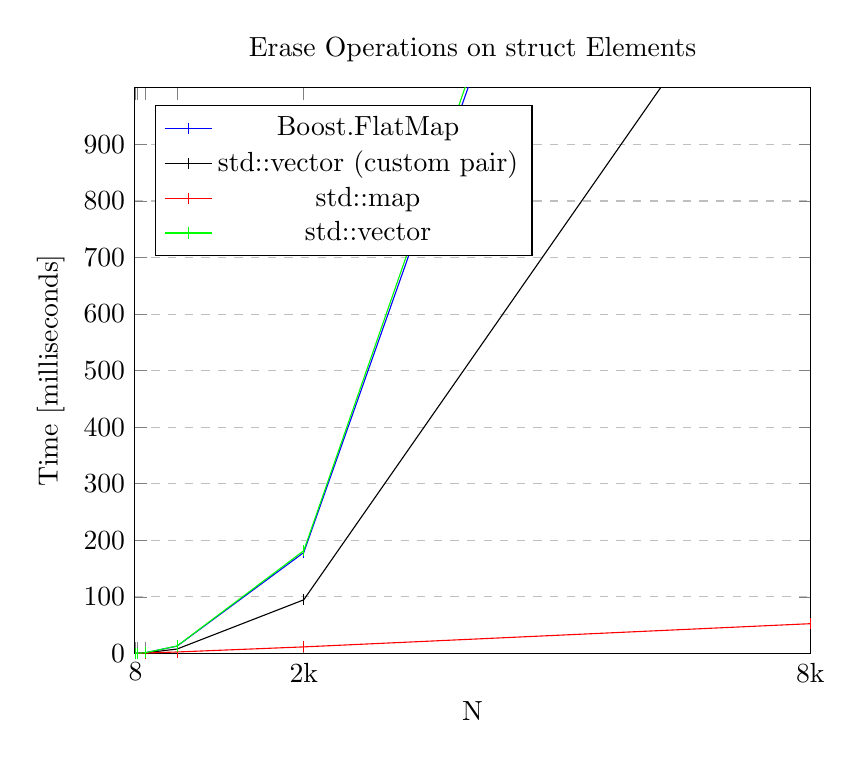
\begin{tikzpicture}
    \begin{axis}[
        width=4in,
        title={Erase Operations on struct Elements},
        xlabel={N},
        ylabel={Time [milliseconds]},
        xmin=0, xmax=8192.0,
        ymin=0, ymax=1000.0,
        xtick={8,32,128,512,2048,8192},
        xticklabels={8,,,,2k,8k},
        ytick={0.0,100.0,200.0,300.0,400.0,500.0,600.0,700.0,800.0,900.0},
        legend pos=north west,
        ymajorgrids=true,
        grid style=dashed,
        scaled x ticks=false,
        legend entries={Boost.FlatMap,std::vector (custom pair),std::map,std::vector},
        ]

    \addplot[color=blue,mark=|,]
        coordinates {(8,0.038063)(32,0.165244)(128,1.1623)(512,12.7604)(2048,178.236)(8192,2711.97)};

    \addplot[color=black,mark=|,]
        coordinates {(8,0.025981)(32,0.135702)(128,0.833067)(512,7.66222)(2048,94.6428)(8192,1380.28)};

    \addplot[color=red,mark=|,]
        coordinates {(8,0.030521)(32,0.122502)(128,0.541619)(512,2.42489)(2048,11.4262)(8192,52.4469)};

    \addplot[color=green,mark=|,]
        coordinates {(8,0.036318)(32,0.159378)(128,1.17312)(512,13.0225)(2048,181.464)(8192,2753.11)};

    \end{axis}
\end{tikzpicture}
\end{center}


TODO
